\chapter{Literature review}
\section{Introduction}
Alzheimer’s disease (AD) is the most common neurodegenerative disease and a leading cause of dementia in the elderly \citep{andrieu2015}. This disease is characterized by a progressive loss of synapses and neurons in certain brain regions (e.g. cerebral cortex and hippocampus), leading to impaired memory and deterioration of cognitive functions \citep{dekosky1990,scheff2006,zare-shahabadi2015}, thus necessitating full-time medical care \citep{prince2013}. Currently the disease is incurable. Although a lot of efforts have been directed towards developing AD disease modifying therapies, current treatment strategies are aimed at ameliorating disease symptoms alone \citep{anand2014,disanto2013}. Age is the most prominent risk factor for AD and about 44 million people are currently affected globally. While only 5\% of individuals over the age of 65 years are affected by AD, the prevalence doubles with every 5 years of increasing age \citep{pimenova2018,qiu2009}. Given the rapidly aging population in first-and third- world countries, the prevalence of AD is predicted to rise to 81 million by 2025 \citep{AlzheimersAssociation2014,Ferri2005}. Moreover, it has been estimated that by 2050, 22\% of the global population will be over the age of 60, with the majority residing in the developing nations \citep{Annear2015,Paddick2013}. In South Africa, there is limited statistics on the prevalence of AD. According to the census conducted in 2011, there are approximately 2.2 million people with some form of dementia. Very little is known about the prevalence of dementia and how it impacts on older adults residing in low and middle classes, as well as in the rural areas, where most of the adult population reside. Despite of this, it was reported that about 79\% of patients were being cared for by family members \citep{Kalula2010}. In the continued absence of effective therapeutic strategies to either delay or slow down the disease progression, AD will pose a tremendously burden on the healthcare and social services. 

AD is a multifactorial disease that is highly complex, with genetic as well as and environmental causes \citep{Dorszewska2016}.This disease is classified into two subsets. The first being the early-onset Familial Alzheimer’s disease (FAD, onset $<$ 65), which contributes to the least cases of AD (1-5\%) with strong genetic association \citep{Musiek2015,Reitz2014,Swerdlow2007}. The second being sporadic late-onset Alzheimer’s disease (LOAD, onset $\geq$ 65) which contributes to the majority of all AD cases ($>$ 95\%), \citep{Musiek2015,Reitz2014,Swerdlow2007}, with an unclear cause \citep{Dorszewska2016,pimenova2018}. Certain genes such as amyloid precursor protein (APP), Presenilin 1 (PSEN1) and Presenilin 2  (PSEN2) are responsible for occurrence of FAD, while APOE gene is responsible for LOAD \citep{Dorszewska2016}.

AD pathology occurs in 5 stages; the pre-symptomatic, Mild Cognitive Impairment (MCI), mild AD, moderate AD and severe AD \citep{Caldwell2015}. The first two stages encompasses a prodromal stage, which, in the majority of cases, precedes symptom onset by several years (at least 20 - 30 years) \citep{Caldwell2015,Caselli2013,Penn1993}. During this time, pathological molecular changes occur inside the brain and are present as two molecular hallmarks which occur as a result of perturbations in cellular proteostasis. The senile plaques, which are extracellular deposits of amyloid beta ($A\beta$)
peptides, and intraneuronal neurofibrillary tangles (NFTs), which are somatic inclusions of hyperphosphorylated, microtubule-associated protein tau, respectively \citep{Mattson2008} (\Cref{fig:10_ad_model}). To better understand the multifactorial pathophysiology of AD, several hypothesis have been put forward, including the amyloid cascade hypothesis (ACH), the cholinergic and tau hypothesis, as well as inflammation \citep{Kurz2011}; however, many molecular aspects and their dynamic changes during disease progression remain unclear. The ACH, the most widely accepted mechanistic hypothesis for AD, posits that an imbalance between the production and clearance of ($A\beta$) peptides is a very early, often initiating factor in disease onset \citep{Hardy2009,Hardy1992}.

\begin{figure}[h!]
  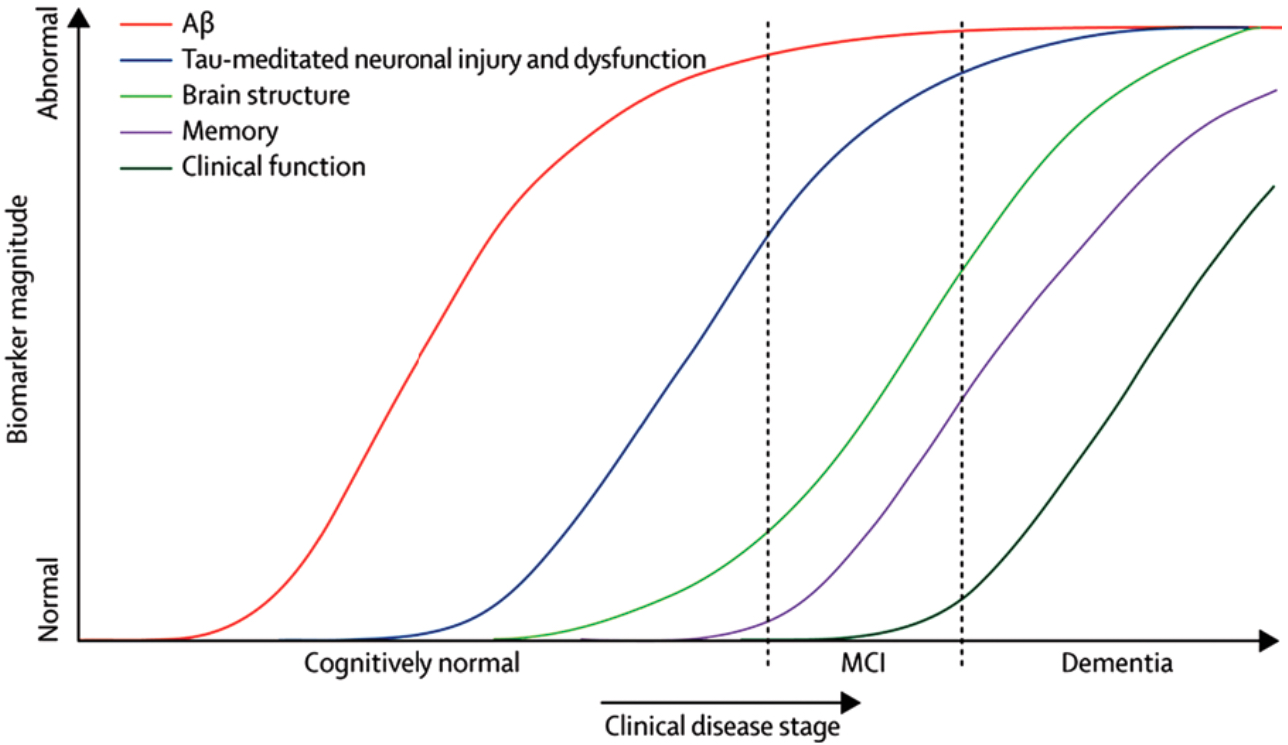
\includegraphics[width=\linewidth]{figures/10_ad_model}
  \caption{Hypothetical model of AD clinical disease stages in relation to biomarkers.  $A\beta$ levels are deposited first and are the initial trigger AD while tau mediated neuronal injury manifests only late in the disease progression, ultimately leading neuronal death \citep{Petrella2013} .}
  \label{fig:10_ad_model}
\end{figure}

Proteolytic systems; the ubiquitin-proteasome system (UPS) and the lysyosomal systems [the autophagy-lysosomal pathway (ALP) and the endocytic- lysosomal pathway (ELP)] are responsible for the degradation of mis-folded or aggregated proteins in order to maintain cellular homeostasis. For example, the UPS targets and degrades short-lived proteins in the cytoplasm and nucleus, while the lysosomal system removes primarily long lived cytoplasmic proteins and damaged organelles \citep{Ravikumar2003,Rubinsztein2005}. A large body of evidence implicates these proteolytic systems in the AD pathophysiology. Dysfunction of these system has been well documented in AD pathophysiology and although extracellular $A\beta$ plaques and intraneuronal NFTs are defining hallmarks of AD neuropathology, a growing body of literature suggests that deficits in the autophagy–lysosomal pathway are likely to precede the formation of these pathological hallmarks \citep{Cataldo2000,Nixon2011,Perez2015,zare-shahabadi2015}, suggesting a potential causality. More recently, a systems biology study highlighted the pivotal role of dysregulated autophagy in neurodegenerative diseases, where toxic protein aggregates and damaged organelles accumulate within specific types of neurons and lead to neuronal dysfunction and ultimately, demise \citep{Caberlotto2014}.

Although we have advanced our understanding of the molecular machinery that regulates the rate of protein degradation through autophagy at basal levels and the many aspects of its dysfunction in AD, the deviation of autophagic activity from basal levels and its change during disease pathogenesis in neuronal tissue remains largely unclear. Over the recent years, we have made substantial progress in modulating autophagy using pharmacological agents \citep{Berger2006,Hebron2013,Ravikumar2002,Ravikumar2004,Rose2010} or lifestyle interventions \citep{Alirezaei2010,Kuma2004,Mizushima2004a,Scott2004} in vitro and in vivo; yet many questions regarding an effective implementation of autophagy control remain unanswered. Therefore understanding the deviation of autophagic activity from basal levels and its change during disease pathogenesis as well as targeting or modulating autophagy activity precisely with the aim to restore autophagic flux may drive the development of better targeted therapeutic interventions that will slow down the disease progression and ultimately curing the disease instead of treating the symptoms. In this review, we start by describing neuronal metabolism and their metabolic profile and move to the involvement of reactive oxygen species in neurodegeneration, focusing on the role of oxidative stress and mitochondrial dysfunction in the pathogenesis of Alzheimer’s disease. We then turn our focus to amyloid beta biogenesis and its pathology in AD.  We highlight the recent advances in the use super resolution techniques in molecular biology. We introduce autophagy and its molecular machinery and discuss its efficiency and essential function in neuronal cells, followed by its role in neurodegenerative diseases. We discuss how autophagic flux may differ in brain regions, and how the deviation of flux may relate to the state of protein aggregation in pathology. Furthermore, we review studies that localize the defect in autophagy in AD and assess the relationship between autophagic flux and neuronal cell death. Finally, we indicate the importance of accurately measuring and targeting autophagy and provide an overview of how autophagy may be modulated for therapeutic purposes in various model systems aimed at restoring autophagic flux. 

\section{Neuronal metabolism}
A brain is made up of two cells types, neurons and astrocytes, which are highly interconnected and form functional networks through their spatial organization. The co-dependency of these cells types is reflected by their metabolic profiles where different yet complimentary pathways are used \citep{Belanger2011,Schonfeld2013} The brain has a high energy demand. This is evident by the fact that 20\% of oxygen and 25\% of the glucose utilized by the human body is dedicated to only cerebral function, yet the brain encompasses only 2\% of the total body mass \citep{Belanger2011}. This means, uninterrupted supply of energy substrates from the circulation is required to meet the energy demands. Glucose is the main substrate of energy in the brain 
\citep{Dienel2012,Pellerin2012} , however, other energy substrates such as lactate, pyruvate, glutamate, and glutamine can be utilized \citep{Zielke2009}.

Glucose is delivered into a cell via specific glucose transporters (GLUTs) and once inside, it is phosphorylated by an enzyme called hexokinase (HK) to generate glucose-6-phosphate (glucose-6P) \citep{Belanger2011,Herrero-Mendez2009}. The latter can enter three main metabolic pathways; glycolysis, pentose phosphate pathway (PPP), and glycogenesis in order to produce adenosine triphosphate (ATP). In glycolysis, glucose-6P is metabolized to produce pyruvate, 2 ATP molecules and NADH \citep{Belanger2011}. Pyruvate can be metabolised further in the tricarboxylic acid (TCA) cycle and oxidative phosphorylation (OxPhos) in the mitochondria using oxygen to generate 30-34 ATP molecules and CO2 or it can be reduced to lactate by lactate dehydrogenase (LDH) in the cytosol \citep{Belanger2011}. In PPP, glucose-6P is metabolized to generate NADPH, while it is stored as glycogen in glycogenesis, with the latter occurring in astrocytes \citep{Belanger2011} (\Cref{fig:10_glucose_metabolism}). More importantly, astrocytes and neurons have the ability to oxidized glucose and/or lactate \citep{Zielke2009}.

\begin{figure}[h!]
  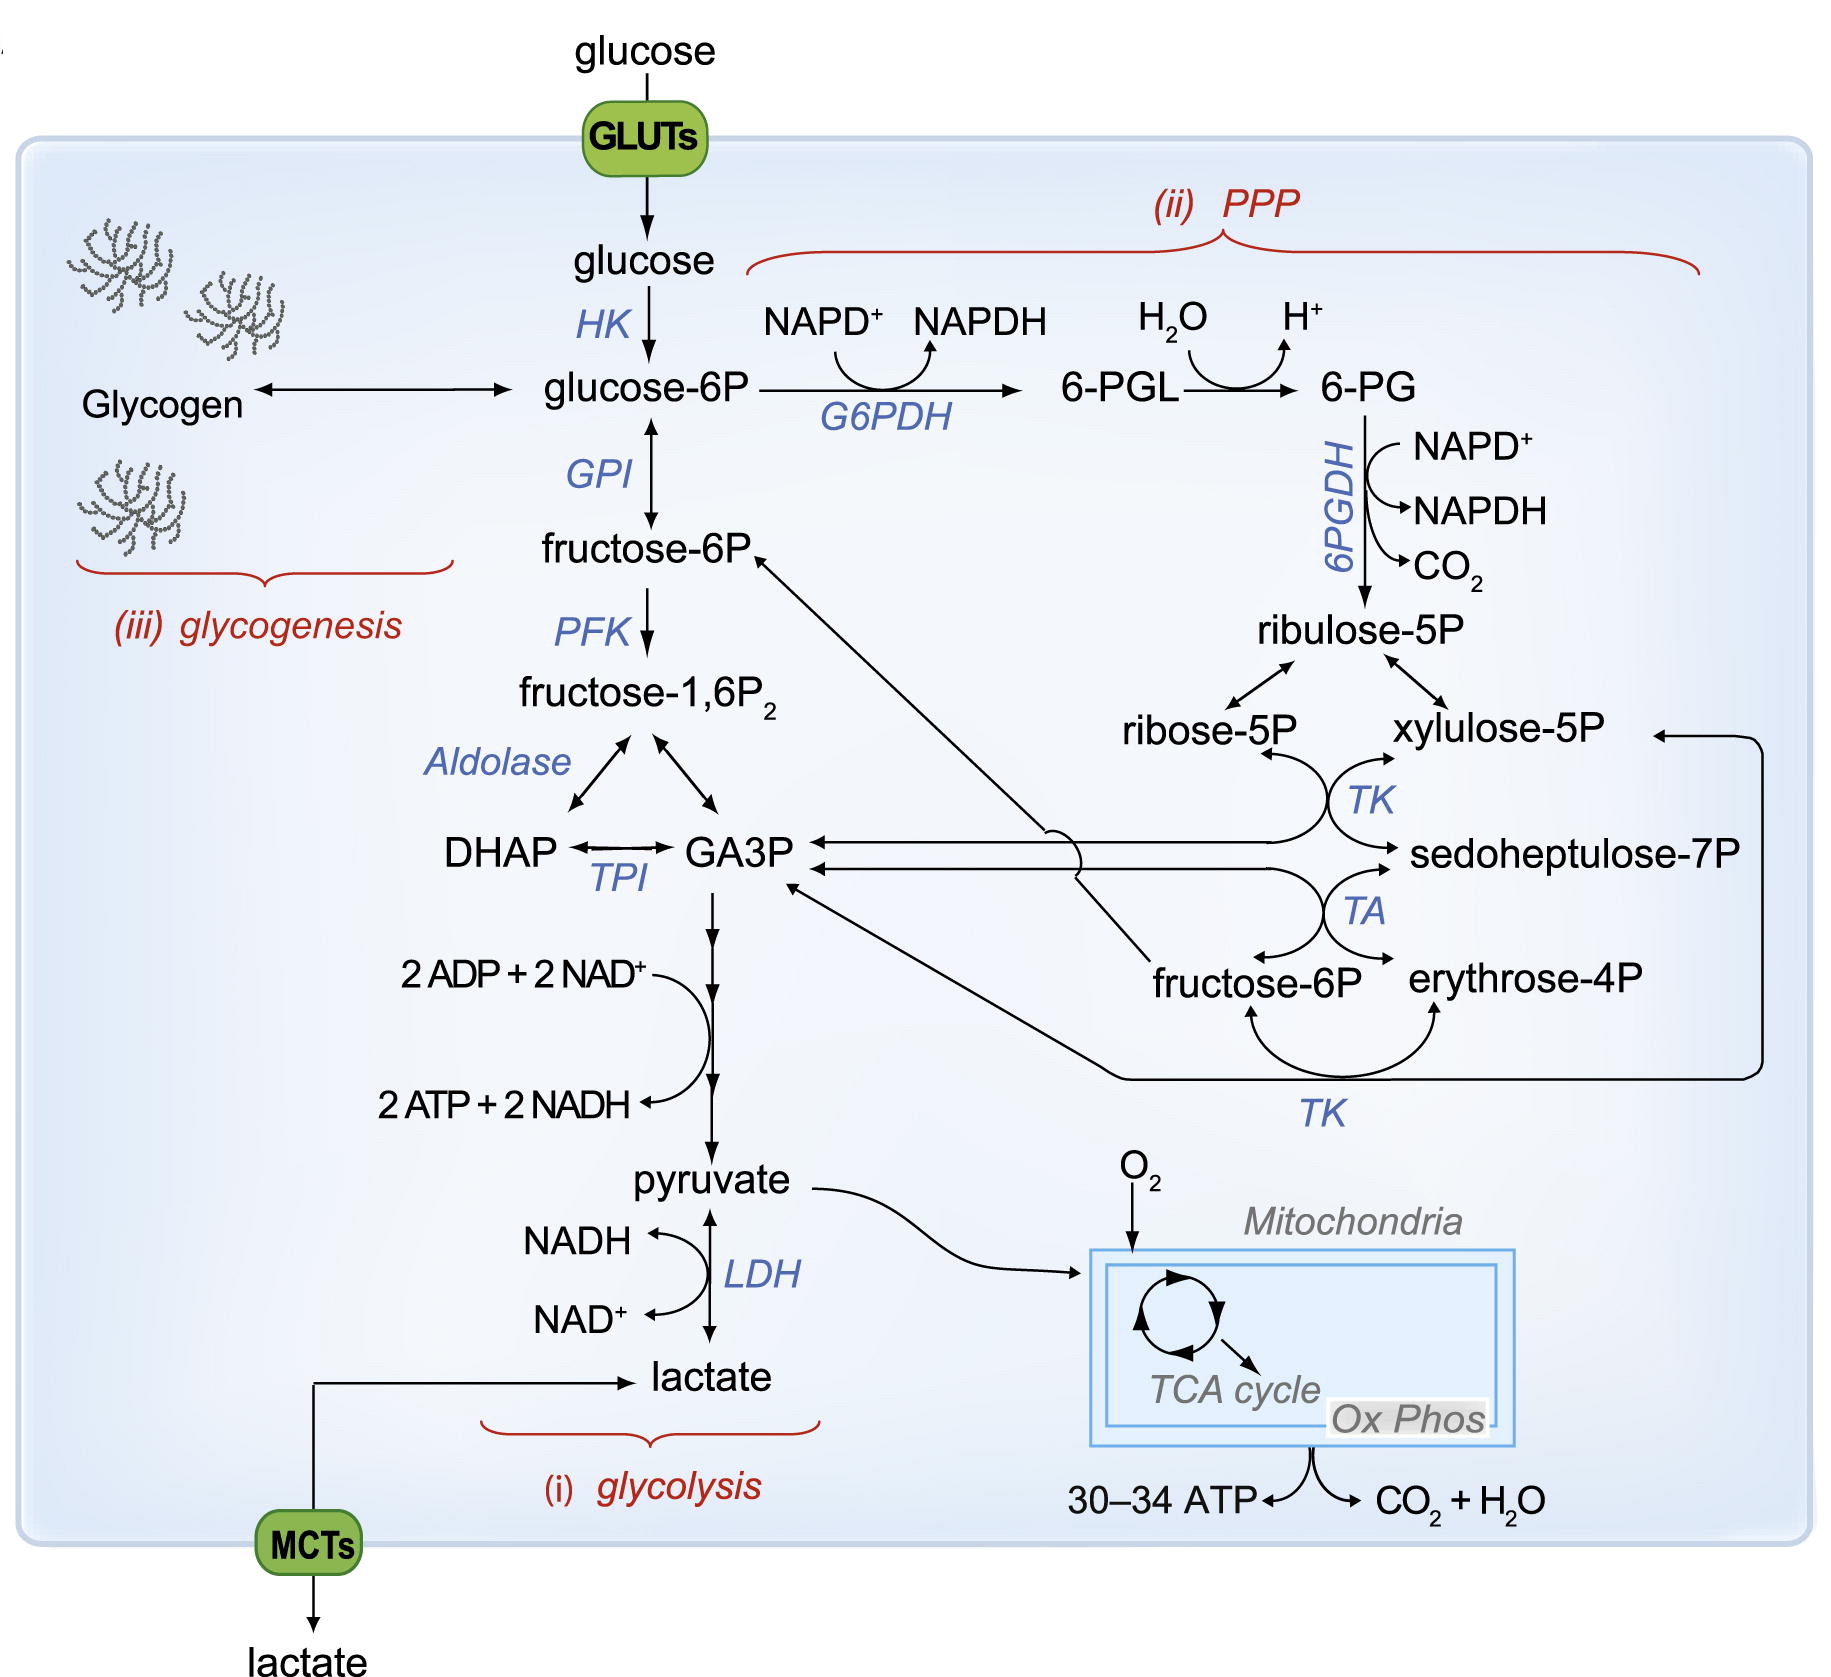
\includegraphics[width=\linewidth]{figures/10_glucose_metabolism}
  \caption{Glucose metabolism. A schematic diagram showing three main pathways; glycolysis, pentose phosphate pathway, and glycogenesis where glucose can be metabolized \citep{Belanger2011} .}
  \label{fig:10_glucose_metabolism}
\end{figure}

\subsection{Metabolic profile of neurons}
Neurons are post-mitotic, highly differentiated cells that are characterized by high energy demands. This is because of their high levels of protein synthesis, which consumes high amount of ATP within the mammalian cells \citep{Buttgereit1995}. Neurons depend almost exclusively on the energy produced through OxPhos (30 - 34 ATP molecules) compared to glycolysis (2 ATP) in order to meet their high energy demand needed to perform cellular functions, such as synaptic plasticity and neurotransmitter synthesis \citep{Cenini2019,Mattson2008,Schonfeld2013}. Mounting evidence demonstrate that neurons are capable of using lactate as an energy substrate \citep{Boumezbeur2010,Bouzier2000,Serres2005} and prefer lactate over glucose when both substrates are available \citep{Bouzier-Sore2006,Itoh2003}. Thus the specific characteristics of neurons are probably underly their distinct metabolic profile. For example, glycolytic enzyme 6-phosphofructose-2-kinase/fructose-2, 6-bisphosphatase-3 (PFKFB3) is highly expressed in astrocytes, but virtually absent in neurons because of a constant proteasomal degradation \citep{Almeida2004,Herrero-Mendez2009}. Because of this, neurons unlike astrocytes display a lower glycolytic rate, and thus cannot upregulate this pathway in response to cellular stress \citep{Almeida2004,Herrero-Mendez2009}. Indeed, a previous study showed that upregulation of glycolysis via PFKFB3 in neurons is in fact detrimental, resulting to oxidative stress and apoptosis \citep{Herrero-Mendez2009}. In this study, it was though that the upregulation of glycolysis occurs at a cost of PPP metabolism that is needed to produce NADPH, an antioxidant vital for maintaining cellular redox state \citep{Herrero-Mendez2009}. Evidently, it has been shown that neurons have low NADPH compared to astrocytes \citep{Ben-Yoseph1996,Garcia-Nogales2003}, and since antioxidant system and the related enzymes are important for maintaining neuronal integrity and survival by keeping the levels of reactive oxygen species (ROS) relatively low \citep{Cenini2019}, it is not surprising that neurons are vulnerable to oxidative damage, implicated in neurodegeneration

\section{ROS and its role in neurodegeneration}
ROS are a group of reactive molecules that produced naturally in biological systems as part of normal cellular metabolism and are important in maintaining cellular homeostasis \citep{Cenini2019}. These include superoxide (O\textsubscript{2}\textsuperscript{-}), hydroxyl radical ($\cdot$OH), hydroxyl ion (OH\textsuperscript{-}) and hydrogen peroxide (H\textsubscript{2}O\textsubscript{2}), all of which are generated from oxygen. O\textsubscript{2}\textsuperscript{-} is generated from O2 in the mitochondria as a result of the respiratory chain complex or NADPH oxidase and can be converted by superoxide dismutase (SOD) enzyme to produce H\textsubscript{2}0\textsubscript{2}. The later  in turn can be converted to other types of ROS, for example OH and OH\textsuperscript{-} \citep{Kim2015a}, with $\cdot$OH being the most reactive ROS responsible for cytotoxicity \citep{Bolisetty2013}.

Under physiological conditions, ROS are maintained at relatively low levels by antioxidant system \citep{Dasuri2013,Gandhi2012}, and are involved cellular processes such as inflammation, immune response, cell survival, synaptic plasticity, learning, and memory \citep{Cenini2019,Kishida2007,Liu2017}. However, increased ROS production can be harmful because of its ability to oxidise nucleic acids, protein and lipids \citep{Wang2014}. Increased ROS accumulation has been implicated in oxidative stress, mitochondrial dysfunction and in gliosis. However, role of ROS in gliosis is poorly understood and only one study provides evidence \citep{Kishida2007}.

Excessive accumulation of ROS due failure of antioxidant system or increased ROS production can result in oxidative stress, an imbalance between rate of ROS production and clearance \citep{Wang2014}. High levels of oxidative stress have been implicated in aging and in the pathogenesis of various neurodegenerative diseases \citep{Bonda2010,Cenini2019,Liu2017,Shibata2008}. Neurons are mostly susceptible to oxidative stress and damage due to its high oxygen consumption, high energy demand, low antioxidant defenses as well as high abundance of polyunsaturated fatty acid which are susceptible to lipid peroxidation \citep{Cobley2018}. Thus, it is not surprising that ROS induced oxidative damage is widely reported in AD. In addition, since mitochondria are the major source of ROS production and the main target of oxidative stress, progressive mitochondrial dysfunction has also been implicated in the pathogenesis of AD \citep{Swerdlow2007}. The involvement of oxidative stress and mitochondrial damage in AD has been demonstrated in different models and are described below. 

\subsection{Evidence of oxidative stress in AD}
Oxidative damage is one of the earliest events in AD \citep{Nunomura2001}. This is supported by several studies that demonstrated elevated levels of oxidative stress in patients with mild cognitive impairment (MCI) \citep{Ansari2010,Pratico2004,Williams2006}. In addition, antioxidants including uric acid, vitamin C and E as well as antioxidant enzymes such as superoxide dismutase (SOD) were found to be decreased in MCI patients \citep{Rinaldi2003,Torres2011}. Increased oxidative stress has also been implicated in AD. Excessive production of ROS is thought to play an essential role in the accumulation and deposition of $A\beta$ peptides \citep{Bonda2010}. \citet{Ferreiro2008} reported that $A\beta$ plaques depleted Ca\textsuperscript{2+} ions storage in the endoplasmic reticulum (ER), leading to in cytosolic Ca\textsuperscript{2+} overload, which resulted in the reduction of endogenous GSH levels and ROS accumulation of ROS. In addition, increased H\textsubscript{2}O\textsubscript{2} levels and increased peroxidation of proteins and lipids were shown in transgenic mouse expressing APP/PS-1, suggesting that $A\beta$ may exacerbate oxidative stress in AD \citep{Matsuoka2001,Zhao2013}. In addition, products of lipid peroxidation such as 4-hydroxynonal (4HNE), malondialdehyde (MDA), and 2 propenal (acrolein) have been found to be elevated in multiple studies performed in patient with AD \citep{Wang2014,Zhao2013}. For example, significantly increased levels of 4HNE were reported in the hippocampus \citep{Lovell1995,Markesbery1998,Montine1998}, parahippocampal gyrus \citep{Markesbery1998}, entorhinal and temporal cortex \citep{Montine1998}, amygdala \citep{Lovell1995,Markesbery1998}, ventricular fluid \citep{Lovell1997}, and plasma \citep{McGrath2001} in AD patients versus control subjects of the same age. Similar findings were observed with MDA and acrolein in AD patients. MDA was found to be increased in the hippocampus \citep{Lovell1995}, pyriform cortex \citep{Lovell1995}, temporal cortex \citep{Marcus1998,Palmer1994} and occipital cortices \citep{Miranda2000}, while elevated levels of acrolein were reported in the hippocampus/parahippocampal gyrus \citep{Bradley2010,Calingasan1999,Lovell2001,Williams2006}, amygdala \citep{Lovell2001},superior and middle temporal gyri \citep{Bradley2010,Williams2006}, and cerebellum \citep{Bradley2010,Williams2006}. Altogether, these studies demonstrate the involvement of oxidative stress in AD

\subsection{Evidence of mitochondrial dysfunction in AD}
As previously mentioned, mitochondria are the main source of oxidative damage due to the continuous generation of superoxide anion that results from electron leakage during electron transfer. Although mitochondria have an efficient antioxidant system, the production of superoxide anions is responsible for 90\% of the endogenous ROS \citep{Wang2014}. It has been suggested that impaired mitochondria are more efficient producers of ROS, but less efficient producers of ATP. In fact, reduced energy metabolism in the brain is among one of the well documented abnormalities in AD \citep{Wang2014}. A genome-wide transcriptomic study suggested that decreased cerebral glucose metabolism in AD was associated with reduced expression of neuronal genes encoding subunits of the mitochondrial electron transport chain. In support of this, several studies reported reduced expression of $\alpha$-ketoglutarate dehydrogenase complex, pyruvate dehydrogenase complex, and cytochrome oxidase in AD, which are the key enzymes of oxidative phosphorylation \citep{Chandrasekaran1994,Cottrell2001,Maurer2000}. Due to the role of mitochondria in calcium homeostasis, previous studies reported calcium mishandling i.e. increased calcium overload and decreased reuptake of calcium in fibroblasts of patients with AD \citep{Ito1994,Peterson1985}. \citet{Area-Gomez2012} reported a significant increase in function of mitochondria-associated ER membranes and ER–mitochondrial communication, measured by cholesteryl ester and phospholipid synthesis, respectively in patients with familial and sporadic forms of AD \citep{Area-Gomez2012}. Consistent with this, ER–mitochondria interface proteins were found to be highly expressed in early stage of AD in patients with AD as well as in the mouse model of APP\textsubscript{Swe/Lon}. Lastly, elevated oxidative damage to mitochondrial DNA was reported in patients with AD \citep{Mecocci1994,Wang2005}. Taken together, these studies provide evidence of the involvement of mitochondrial dysfunction in AD.

\subsection{Role of PQ in oxidative stress and in the pathogenesis of AD}
PQ is a pesticide that is widely used globally for agricultural practices. Several epidemiological studies have reported that pesticide exposure increases the risk of developing AD \citep{Baldi2003,Hayden2010,Santibanez2007,Yan2016}. In fact, genetic factors and environmental factors are the aetiology of the sporadic form of AD \citep{Landrigan2005}. Although the mechanism of PQ are better understood PD than in AD, it is known that PQ accumulates in the cerebral cortex and hippocampus \citep{Landrigan2005}. Therefore, PQ could potentially impair learning and memory functions and affect AD pathogenesis. PQ exact its toxicity by inducing oxidative stress and mitochondrial damage \citep{Baltazar2014,Drechsel2008,Lin2006}, both of which are implicated in the pathogenesis of AD \citep{Lin2006}. Therefore, experimental models with PQ are widely used for understanding the roles of pesticide exposure in the development of AD as well as to study the mechanisms of AD. \citet{Drechsel2008} showed that PQ enhances H\textsubscript{2}O\textsubscript{2} production in brain mitochondrial. Since H\textsubscript{2}O\textsubscript{2} is essential for regulating redox-sensive signaling under normal condition \citep{Rhee2006}, it is not surprising that its increased generation from the mitochondria has been implicated in the development of AD \citep{Du2008,Manczak2006}. In another study, exposure to PQ was found to increase oxidative stress measured with 4HNE and nitrotyrosine levels in the mitochondria of cerebral cortex and to exhibit mitochondrial dysfunction in wild-type mice and APP transgenic mice \citep{Chen2012}. The authors also reported an increase in mitochondrial damage which was found to be directly correlated with impaired learning and memory as well as elevated $A\beta$ levels \citep{Chen2012}. Moreover, it was reported that overexpression of peroxiredoxin 3, a mitochondrial antioxidant defense enzyme, whose role is to remove H\textsubscript{2}O\textsubscript{2} in the mitochondria protected against PQ induced mitochondrial damage, while decreasing $A\beta$ levels and improving cognition \citep{Chen2012}. These results suggest the importance of H\textsubscript{2}O\textsubscript{2} in the pathogenesis of AD.

\section{$A\beta$ biogenesis}
Amyloid precursor protein (APP), an evolutionary conserved type 1 transmembrane protein, is unequivocally linked to AD pathogenesis as the unique source of neurotoxic forms of $A\beta$ \citep{Chen2015,Rajendran2012}. During early development, APP is highly enriched at the growth cones of developing neurites \citep{Ramaker2016,Sabo2003}. In more mature neurons, APP localizes to focal adhesion sites and within pre- and postsynaptic structures of the central and peripheral nervous tissue, suggesting a functional role in neuritic growth and synaptic plasticity \citep{Ashley2005,Yamazaki1997}. APP is synthesized in the ER and transported to the Golgi apparatus where it is packaged into vesicles for delivery to the cell surface for further processing by $\alpha$-, $\beta$-, and $\gamma$-secretases following the non-amyloidogenic (constitutive) or amyloidogenic pathway (\Cref{fig:10_amyloidogenic_pathway}) \citep{Obrien2011,Ramaker2016}. The cleavage activity of the $\beta$, and $\gamma$-secretases is mediated by the  $\beta$-site APP-cleaving enzyme 1 (BACE1) and presenilins (PSENs) catalytic domain, respectively \citep{Rajendran2012}. 

The non-amyloidogenic pathway leads to the production of non-pathogenic fragments, while the amyloidogenic pathway promotes the generation of $A\beta$ peptides. Briefly, following the former pathway, APP is first cleaved by $\alpha$-secretase also known as distintegrin or metalloproteinase 10 (ADAM10), within the $A\beta$ sequence, thereby blocking $A\beta$ production, to generate two proteolytic fragments: soluble APP$\alpha$, and the corresponding C-terminal fragments, $\alpha$-CTF/C83 (a protein stub that remains secured to the plasma membrane for further proteolytic processing) \citep{Gandy1994,Roychaudhuri2009}. Soluble APP$\alpha$ is recycled back to the cell surface by the recycling compartments or delivered to the lysosome for degradation through the endosomal– lysosomal system \citep{Caster2013,Golde1992}. In the amyloidogenic pathway, APP is cleaved by $\beta$-secretase, the major secretase in the brain, at the N-terminus of the $A\beta$ sequence, thus generating soluble APP$\beta$, which is released extracellularly, and the corresponding C-terminal fragment, $\beta$-CTF/C99 (a membrane-associated fragment comprising the entire $A\beta$ sequence). Both C99 and C83 are subsequently cleaved by $\gamma$-secretase within the transmembrane domain, resulting in the release of a nontoxic p3 fragment, APP intracellular domain, and $A\beta$ peptide species of slightly different lengths (\Cref{fig:10_amyloidogenic_pathway}) \citep{Cole2007,Jarrett1993}. Secretase cleavage gives rise to an admixture of $A\beta$ peptides composed of 39–43 amino acids, with $A\beta$40 (90\%) and $A\beta$42 (10\%) being the two major $A\beta$ species \citep{Gouras2000,Takahasi2013}. Neuronal cells produce both $A\beta$40 and $A\beta$42 peptides, with healthy neurons having a high $A\beta$40/$A\beta$42.

\subsection{Role of $A\beta$ pathology in AD}
Although $A\beta$42 is produced at low quantities in neurons, it has a higher tendency to self-aggregate and form higher order structures, including toxic $A\beta$ dimers, trimers, and oligomers. These higher order structures able to coalesce to form fibrils in insoluble beta-sheet conformation that eventually deposit into diffuse senile plaques \citep{Burdick1992,Gravina1995}. However, various studies have shown that the oligomers are main source of its neurotoxicity \citep{Shankar2008,Shankar2009}. Although autophagy is responsible for the bulk degradation of aberrant proteins, not all aggregate-prone proteins are fully amenable to autophagic degradation \citep{Wong2008}. For example, expression of human $A\beta$40 and $A\beta$42 in Drosophila brain has been shown to have differential effects on neuronal autophagic degradation {Ling2009}. Studies have shown that although autophagy sequesters $A\beta$42, this aggregate-prone peptide in turn may decrease the degradative capacity of autophagy \citep{Ling2014,Ling2011}. This was demonstrated by highly concentrated intracellular $A\beta$ identified in autophagic vacuoles (AVs), which accumulate in affected neurons, especially with advancing age \citep{Ling2011}. In contrast, sequestration of $A\beta$40 does not produce any detectible changes in either the neuronal autophagy activity or neurological defects in vivo, which is consistent with the ACH for AD pathogenesis \citep{Hardy1992}.

Prior to senile plaque deposition, $A\beta$42 oligomers are able to induce oxidative damage, promote tau hyperphosphorylation, and lead to synaptic and mitochondria toxicity (\Cref{fig:10_amyloidogenic_pathway}) \citep{Kaminsky2015,Lustbader2004}. Moreover, during late disease progression, $A\beta$42 senile plaques have been found to activate microglia \citep{Rosenmann2013}. Microglial activation results in the production and release of proinflammatory cytokines, including IL-1$\beta$, TNF-$\alpha$, and IFN $\gamma$, which in turn stimulate the nearby astrocytes to further exacerbate $A\beta$42 production and dispersal \citep{DalPra2015}. To this end, immunohistochemical analysis has revealed significantly higher $A\beta$42 levels in AD brains than control brains \citep{Funato1998}. Additionally, the extent of $A\beta$42 deposition is much greater in AD brains with disease progression, while $A\beta$40 shows little or no apparent age-dependent accumulation \citep{Funato1998}.

It is well established that AD-causing mutations in APP and in presenilin 1 (PSEN1) and presenilin 2 (PSEN2) alter APP proteolytic processing in a manner that alleviates the relative levels of the $A\beta$42 peptides \citep{Borchelt1996,Scheuner1996}. Mutations in APP that lie within the $A\beta$ sequence increase the self-aggregation of the resultant peptides, not their production, while mutations in PSEN1 and PSEN2 increase the relative production of the longer, more hydrophobic, and self-aggregating $A\beta$42 peptides \citep{Kim2008,Weggen2012}. Furthermore, the inactivation of PSEN1 and PSEN2 has been shown to completely prevent $A\beta$ generation \citep{Herreman2000,Zhang2000}. Although $A\beta$42 is generated at a 10-times lower rate than $A\beta$40, the former peptide has consistently been shown to be the main component of $A\beta$ plaques in AD \citep{Iwatsubo1994}. Originally, the ACH was mostly driven by genetic studies indicating the vast majority of early-onset familial AD mutations to confer a similar biochemical phenotype, i.e., an increased ratio of cerebral $A\beta$42, either through an increased $A\beta$42 production or decreased $A\beta$40 production, or a combination of both \citep{Cavallucci2012,Cruts1998}. And although the ACH takes a central position in AD-related research, the prevailing hypothesis does not entirely account for the complex pathophysiology of AD. Instead it seems that the role of $A\beta$ in synaptic degeneration may act in concert with several other factors that impair the integrity of neuronal functions \citep{anand2014,DalPra2015}. Growing evidence supports that dysregulated production of both $A\beta$ and tau may synergistically disrupt synaptic activity and mitochondrial function, resulting in AD \citep{Chetelat2013,Musiek2015,Quintanilla2012,Teplow2013}. Although many factors contribute to AD pathogenesis, imbalance in $A\beta$ production and clearance has emerged as the most extensively validated and compelling therapeutic target for both genetic and sporadic AD, as both forms of the disease can be ascribed similar etiologies \citep{Selkoe2012,Selkoe2016}.

\begin{figure}[h!]
  \center
  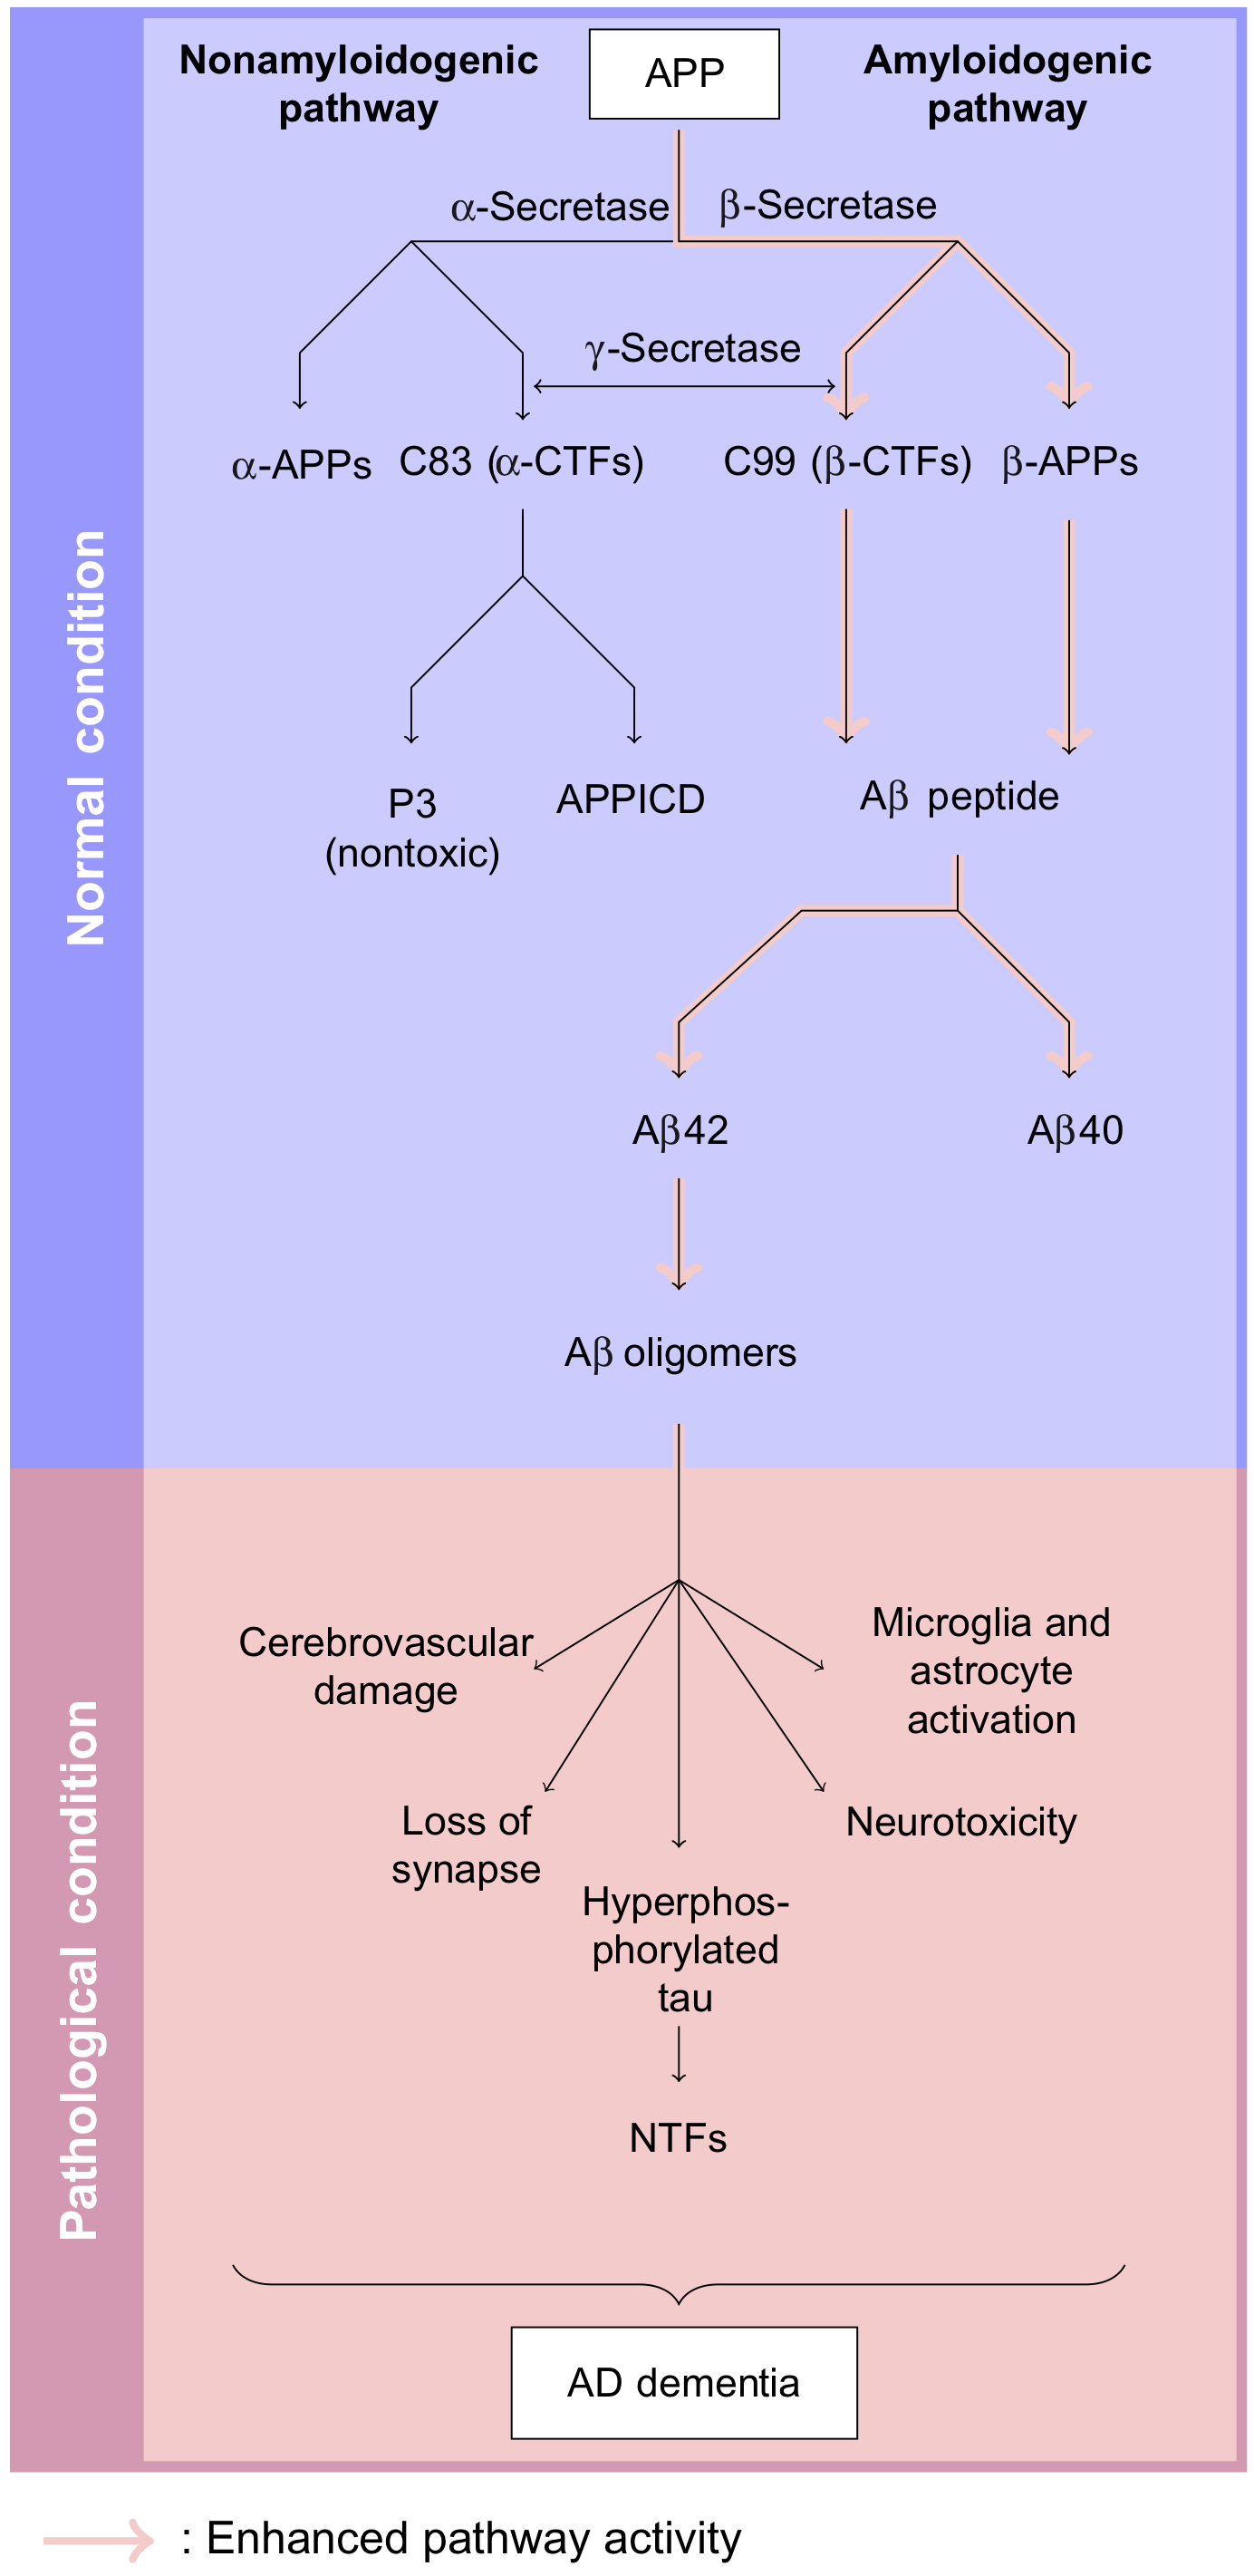
\includegraphics[width=0.7\linewidth]{figures/10_amyloidogenic_pathway}
  \caption{The nonamyloidogenic and amyloidogenic pathways. Enhanced amyloidogenic pathway activity increases neuronal synthesis of aggregate prone toxic $A\beta$ oligomers, which in turn lead to autophagy and mitochondrial dysfunction as well as tubulin disruption, thereby driving neurofibrillary tangle (NFT) formation}
  \label{fig:10_amyloidogenic_pathway}
\end{figure}

\section{Advanced microscopy in the study of molecular biology}
\subsection{Role of super-resolution microscopy }

Microscopes play a key role in molecular biology. Fluorescence microscopy in particular remain one of the most important tools for biologists for various reasons. Firstly, it is essential for studying communications of biological molecules inside living cells, tissues, and whole organisms and subcellular structures at high resolution \citep{Han2013}. Secondly, it can acquire data rapidly and molecules of interest are targeted and labelled with specific fluorescence probes in a noninvasively manner \citep{Han2013}. Thirdly, live cell imaging is possible. In conventional microscopes, the spatial resolution is limited in diffraction, about 200 nm in the $xy$ and 500 nm in the $z$ direction, making it impossible to identify smaller sub-cellular structures or monitor biological processes which occur at nanometer scale \citep{Xu2017}. Therefore, in the past two decades, efforts to break the diffraction limit in order to understand cell structure and dynamics at a molecular level in 2 or 3 dimensions have been made. Currently, super resolution microscopes capable of imaging cellular structures and rapid cellular dynamics at single molecule level at 10 nm are available. These include stimulated emission depletion (STED) microscopy \citep{Klar1999} and saturated structured illumination microscopy (SIM) \citep{Gustafsson2005} which use patterned illumination to improve the resolution by controlling few molecules which are excited and detected simultaneously and single molecule localization microscopy which work by activating single molecules at different times \citep{Han2013} such as  photoactivation localization microscopy (PALM) \citep{Betzig2006} and stochastic optical reconstruction microscopy (STORM) \citep{Huang2008,Xu2017}, \Cref{fig:10_superresolution}. The application of these techniques in molecular biology has been extensively reviewed elsewhere \citep{Han2013}. For the purpose of this review, we focus on single molecule localization techniques.  

Briefly, STORM/PALM is based on the photo switching and detecting single spatially separated fluorophores. This is achieved by photoswitching  fluorophores between their  "ON" and "OFF" state, where most of the them are forced to remain in the dark state for a longer time and allowing on only a small subset of fluorophores  in  the “on” state to emit fluorescence at a given time \citep{Turkowyd2016}. In this manner, thousands of frames are imaged overtime  and reconstructed using image-processing algorithms allowing the precision localization of molecules, which depended on the sufficient collection of photons from each activation event and therefore, the reliability of the fluorophores employed \citep{Turkowyd2016,Xu2017}.

Currently, the use of correlative techniques such as correlative light and electron microscopy (CLEM) is gaining popularity in molecular biology. CLEM is a unique and powerful technique that combines two different imaging modalities, fluorescent light microscopy (LM) and electron microscopy (EM) in order to overcome the limitations of each, however at an expense of imaging fixed sample \citep{Russell2017}. Light microscopy allows one to identify fluorescently labelled molecules for their biological function within living cells and tissues which would not have been possible with TEM however the information is limited in resolution 200nm or 10 nm with advanced super-resolution microscopy.  EM on the other hand allows ultrastructural visualization at a much fine resolution, 0.1 -10 nm \citep{Feng2018}, thus combining these techniques has makes it possible for imaging image  rare dynamic biological events at high resolution. CLEM has undergone a dynamic evolution. Traditionally, it was performed using TEM on manual sectioned serial sections and imaging each section (more than 100 sections) using TEM. Nowadays, automated systems  based on the SEM such as focused ion beam SEM (FIB-SEM) \citep{Heymann2006} and serial blockface SEM (SBF-SEM) \citep{Denk2004} have gained popularity and are being used molecular biology. In FIB-SEM and SBF-SEM, a gallium ion beam  or a diamond knife is used to sputter or remove slices of material from the blockface and the revealed surface is imaged repeated sequentially using a backscattered electron (BSE) detector to build up a stack of images through the volume of the sample \citep{Russell2017}

\begin{figure}[h!]
  \includegraphics[width=\linewidth]{figures/10_superresolution}
  \caption{Super-resolution fluorescence microscopy. Diagram showing the principles of super-resolution microscopy techniques (upper panel) and images  of microtubules imaged with each microscopy (lower panel) \citep{Feng2018}.}
  \label{fig:10_superresolution}
\end{figure}

\section{Autophagy}
\subsection{Definition and role}
Autophagy is a major catabolic process responsible for the degradation cytoplasmic material, including organelles within the lysosomal compartment \citep{He2009,Nixon2011}. Three types of autophagy exist, depending on the route through which the encircled cargo is delivered to the lysosomal compartment for degradation: microautophagy, chaperone-mediated autophagy (CMA), and macroautophagy \citep{Boya2013}. In microautophagy, cytosolic components are directly transferred into the lysosomes through invagination of the lysosomal membrane \citep{Cai2012,Nixon2011}. In CMA, the protein targeted for degradation is recognized by a chaperone complex protein, HSC70, through a KFERQ motif located on the target protein peptide sequence. Subsequently, the substrate-chaperone complex is transported to the lysosome where it binds to the lysosome associated membrane protein type 2A (LAMP-2A) receptor allowing the translocation of the protein across the lysosomal membrane into the lumen, where it is degraded \citep{Cuervo2014,Dice2007,Klionsky2010}. And lastly, macroautophagy (here after referred to as autophagy) which is the major degradation pathway of long-lived proteins and organelles, which operates entirely different compared to microautophagy and CMA, through distinct and dynamic membrane rearrangements. Here, a flat membraned cistern known as the phagophore sequesters substrates. The membrane source of phagophores is believed to arise from the  endoplasmic reticulum (ER), plasma membrane, mitochondria and ER-mitochondria contact sites \citep{Hailey2010,Hamasaki2013,Hayashi-Nishino2009,Ravikumar2010,sarkar2013,Yla-Anttila2009}.
The phagophore elongates and encircles the cytoplasmic material, forming a double-membraned vesicle, called an autophagosome \citep{Cai2012,Levine2008}, which subsequently fuses with lysosomes or with late endosomes to form a single-membrane hybrid organelles, amphisome, that latter fuses with lysosomes to form acidic autolysosome \citep{Cai2012,Nixon2011,sarkar2013}, where degradation of the encircled cargo takes place (\Cref{fig:10_macroautophagy}). The resulting macromolecules are recycled back into the cytosol to be reused as substrates for ATP generation or protein synthesis. The rate of protein degradation through autophagy is termed autophagic flux \citep{klionsky2016,loos2014}. Importantly, most cells and tissues have a distinct basal level of autophagic flux \citep{Mizushima2004a}, which has recently been elegantly visualized in various tissues \citep{Kaizuka2016}. Autophagy therefore plays a critical role in maintaining cellular homeostasis by removing misfolded or damaged proteins and turnover of organelles \citep{Levine2008}. It also plays a role in maintaining energy homeostasis during starvation conditions by recycling cytosolic components to compensate for nutrient scarcity \citep{Levine2008,Loos2009}. Although autophagy play a major role in cellular survival, it has been implicated in various human physiological and pathological conditions, such as development, aging, infection and immunity, longevity, aging, cancer, liver, neurodegeneration and heart disease \citep{Meijer2006,Mizushima2008,Ravikumar2010b,sarkar2013}.

\begin{figure}[h!]
  \includegraphics[width=\linewidth]{figures/10_macroautophagy}
  \caption{The multistep pathway forming an energetic loop from energy sensing to cargo degradation and amino acid release.}
  \label{fig:10_macroautophagy}
\end{figure}

\subsection{The autophagic machinery and its regulation}
Autophagy is evolutionarily conserved from yeast to mammals with up to 36 ATG (autophagy-related genes) \citep{Thumm1994,Tsukada1993,Klionsky2007,Mizushima2010}. Subsets among these ATG proteins referred to as the ‘core’ molecular machinery are essential for autophagosome formation. These are classified into four groups; (1) the ULK1 kinase complex, (2) ATG9 cycling complex, (3) the class III phosphatidylinositol 3-kinase (P3K)/ Vps 34 complex I, (4) the phosphatidylinositol 3-phosphate (PI3P) binding ATG2-ATG18 complex and (5) ATG12-ATG5 and ATG8/LC3 (microtubule-associated protein 1 light chain 3) \citep{Feng2014,Yang2010}.

The autophagic pathway can be categorized into the following essential steps: initiation, expansion of the autophagosome membrane, maturation of the autophagosomes, and degradation. Each step requires tight regulation of several, indispensable, ATG genes (\Cref{fig:10_macroautophagy}) \citep{Feng2014,Maday2014,Parzych2014}. Although the initiation of autophagy is constitutively kept at low levels, diverse environmental stressors (e.g. reactive oxidative species, damaged organelles and protein aggregation) can act as inducers of this degradative machinery \citep{Mizushima2008}. Starvation is the classic stimulus for autophagy induction \citep{Kuma2004,Mizushima2004a}, allowing cells to respond to nutrient scarcity through increased allocation of amino acids from proteins sequestered as autophagic cargo \citep{Hosokawa2009}. The classical pathway regulating mammalian autophagy involves the serine/threonine kinase, mammalian target of rapamycin (mTOR): mTORC1 and mTORC2, in which mTORC1 negatively regulates autophagy \citep{Guertin2009,Noda1998,Ravikumar2010b}. During conditions of nutrient availability, active mTORC1 phosphorylates Unc-51-like kinase (ULK1), which is sequestered into a complex with the autophagic protein, ATG13, and focal adhesion kinase family interacting protein of 200kDa (FIP200), thereby inhibiting autophagy. In the absence of nutrients, amino acid deprivation, growth factor withdrawal, or treatment with rapamycin, ULK1 phosphorylation by mTORC1 is reduced and the ULK1 complex is activated through auto-phosphorylation, which in turns phosphorylates ATG13 and FIP200.  Activated ULK1 phosphorylates and activates the Beclin1-vacuolar protein sorting 34 (VPS34) complex, which contains Beclin1, VPS34, and Atg14L \citep{Itakura2008}. The activated Beclin1 complex functions as a class III phosphatidylinositol 3-kinase (PI3KCIII), to produce phosphatidylinositol 3-phosphate (PI3P), which in turn provides a platform to recruit PI3P-binding proteins during the nucleation process \citep{Hosokawa2009,Kim2011,sarkar2013}. Atg14L targets the Beclin1/PI3KCIII complex to the specialized subdomain of the endoplasmic reticulum (ER), called the omegasome, which consequently triggers phagophore formation \citep{Axe2008,Matsunaga2010}. Although the Golgi apparatus, mitochondria and plasma membrane may also act as membrane sources for phagophore formation under certain conditions \citep{Axe2008,Ravikumar2010}, a growing number of studies have revealed that phagophores locate between two cisterns of rough ER in starved cells \citep{Hayashi-Nishino2009,Yla-Anttila2009}. In support of this, the omegasome marker protein DFCP1 was found to be localized in delicate membrane tubules extending from the ER, thus making the ER the most likely membrane source for the formation of phagophores \citep{Uemura2014}. Beclin1 has many binding partners such as Atg14L, UV-irradiation- resistance-associated gene (UVRAG), and Bcl2 \citep{He2010}.

Positive regulators of Beclin1 function and autophagy include AMBRA1, UVRAG and Bif-1; and negative regulators include the anti-apoptotic proteins Bcl2 and BCL-XL \citep{Pattingre2005,Sinha2008}. Bcl2 inhibits autophagy indirectly through its interaction with Beclin1 \citep{Pattingre2005}. This Bcl2 modulation aims to prevent excessive degradative activity of the cells and subsequent cell death \citep{Pattingre2005}. Positive UVRAG association with Beclin1 has been shown to enhance PI3KCIII activity and induces autophagosome formation \citep{Liang2006}. In addition to this, Beclin1 is also involved in various pathophysiological processes associated with neurodegeneration \citep{He2010}. Its functional role within the PI3KCIII complex is especially important for cellular homeostasis, as it maintains the dynamic coordination of specific endosomal trafficking and autophagy steps (e.g., initiation and nucleation) \citep{Liang2008,Matsunaga2009,Russell2013}. For example, Beclin1 has also been found to restore autophagic activity in ATG6-disrupted yeast, becoming one of the first identified genes to positively regulate autophagy \citep{Liang1999}.
